\documentclass[10pt,a4paper]{article}
\usepackage[margin=2cm]{geometry}
\usepackage{amsmath,amssymb,bm}
\usepackage{booktabs,tabularx,multirow,array}
\usepackage{enumitem}
\usepackage[table]{xcolor}
\usepackage{graphicx}
\usepackage{tikz}
\usetikzlibrary{positioning,arrows.meta,fit,backgrounds,calc,shapes.geometric}
\usepackage[numbers,sort&compress]{natbib}
\usepackage{hyperref}
\usepackage{caption}
\usepackage{subcaption}
\usepackage{float}
\hypersetup{colorlinks=true,linkcolor=blue!50!black,citecolor=green!35!black,urlcolor=blue!50!black}
\setlist{nosep,leftmargin=1.4em}
\captionsetup{font=small,labelfont=bf}
\newcommand{\code}[1]{\texttt{#1}}
\newcommand{\R}{\mathbb{R}}
\definecolor{sim}{RGB}{226,238,250}
\definecolor{per}{RGB}{230,244,232}
\definecolor{ctl}{RGB}{252,234,222}
\definecolor{off}{RGB}{242,234,250}
\definecolor{frz}{RGB}{236,236,240}
\definecolor{trn}{RGB}{255,243,205}
\tikzset{box/.style={draw,rounded corners=2pt,align=center,font=\footnotesize,minimum height=9mm,inner sep=3pt},
         arr/.style={-{Latex[length=2mm]},thick}, lab/.style={font=\scriptsize,align=center}}

\title{VLSS: A Semantic-Aware Vision-Language Safety Scorer\\for Risk-Shaped Control Barrier Functions in Mobile Robot Navigation}
\author{Project report}
\date{15 November 2026}

\begin{document}
\maketitle

\begin{abstract}
Safety filters for mobile robots usually treat every obstacle alike: a sofa, a bucket that carries a glass and a person all get the
same clearance. Which obstacle matters depends on what it is and on what it carries, which geometry alone cannot tell, and the
foundation models that can tell are too slow to sit in a control loop. We present VLSS, a vision-language safety scorer that gives
every obstacle in a camera image a semantic risk in $[0,1]$ in a single forward pass, and a model predictive controller whose
control barrier functions are shaped by those risks. Obstacles are segmented by SAM~3 from open-vocabulary prompts; VLSS, a
4-billion-parameter vision-language model with one query token per mask and a regression head, is distilled from a
33-billion-parameter teacher that rates obstacles against a written rubric with privileged scene information, after human review
of the teacher's labels. The risk sets both the margin and the decay rate of a discrete-time barrier, while a hard contact
constraint holds whatever the score. In a simulated environment with two kinds of actor moving a glass, VLSS runs at 29~ms per
frame, is within 0.052 of the reviewed labels on unseen layouts, ranks 99.6\,\% of obstacle pairs correctly, keeps 92\,\% of its
scores inside the policy ranges in a scene with furniture, containers and materials never seen in training, and partly generalises
to an arrangement held out of training. In closed loop with simulator obstacles, semantic risk keeps the robot 0.11~m from the
container that carries the glass instead of 0.01~m, at no cost in time to the goal. The full perception-to-control loop does not
yet reach the goal; we report why.
\end{abstract}


%======================================================================================================================
\section{Introduction}

Mobile robots increasingly share space with people and with things that matter: a care robot in a home passes tables with
glasses on them, a delivery robot in a hospital passes trolleys of instruments, and an autonomous mobile robot in a warehouse or a
factory passes pallets, workers, drums of chemicals and stacks of empty cartons. In all of these places the robot must reach its
goal without touching anything, and when space is short it must decide what to pass close to. Bumping a cardboard box or an
upholstered chair is harmless; bumping a pallet that carries glass bottles, a shelf with a monitor on its edge, or a person is not.

Safety filters based on control barrier functions (CBFs)~\cite{ames2019cbf} and model predictive control~\cite{zeng2021dcbf}
guarantee that a robot stays outside the obstacles they know about, and recent work makes them run on rich geometric scene
representations~\cite{chen2025splatnav,chen2025safersplat,hong2026polymerge,tscholl2025collisioncone}. They treat all obstacles
alike, however: every obstacle gets the same clearance and the same approach rate. The distinction between a sofa and a bucket
carrying a glass is \emph{semantic}. It depends on what an object is, on what stands on it or is held by it, and on whether damage
can be undone, which a depth sensor cannot measure.

Vision-language models (VLMs) know these distinctions, and a growing body of work uses them to decide what is unsafe and to feed
that decision to a safety filter~\cite{brunke2025semantic,ravichandran2026core,feng2025words,santos2025updating,chen2026alphaadj}.
Three difficulties remain. \emph{Latency}: a large VLM takes seconds per image, while a controller needs fresh information several
times a second. \emph{Granularity}: many approaches give one scalar for the whole scene or a fixed list of rules, while the
controller needs a value per obstacle that can change when, for example, a glass is put down on a bucket. \emph{Trust}: a
learned score that is wrong must not lead to a collision.

We address these with a scorer, VLSS (\emph{vision-language safety scorer}), and a controller that uses it:
\begin{itemize}
\item \textbf{A per-obstacle semantic risk scorer at control rate.} VLSS reuses a 4B-parameter VLM, but replaces text generation
by a regression head on one query token per obstacle mask, in the way vision-language-action models (VLAs) replace it by an action
head~\cite{zitkovich2023rt2,kim2024openvla}. One forward pass of 29~ms rates every obstacle in the image, and attention lets each
obstacle's score use the pixels around it: a bucket's score can depend on the glass standing on it.
\item \textbf{A labelling pipeline with a privileged teacher and human review.} A 33B-parameter VLM rates simulated obstacles
against a written rubric; it receives close-ups of each obstacle and the simulator's knowledge of what stands on what, which a
pilot showed it needs. A reviewer corrects the policy on a sample, and the corrections are applied to all labels in a traceable
way before distillation~\cite{hinton2015distilling}.
\item \textbf{Risk-shaped barriers with a risk-independent floor.} In a CBF-NMPC the risk of each obstacle sets both the margin of
a soft discrete-time barrier and its decay rate, while a hard contact constraint does not depend on the score, so a wrong score
changes how cautious the robot is but never permits contact.
\item \textbf{An evaluation of generalisation.} Besides unseen layouts, we test an arrangement held out of training (something
fragile on a support the model never saw carrying anything) and a scene whose furniture, containers and materials the model never
saw, and we report closed-loop results with semantic and uniform risk.
\end{itemize}

The method is not tied to one environment: the obstacle prompts, the rubric and its policy ranges are configuration, and nothing
in the scorer or the controller is specific to the test environment used here, a walled alley in Isaac Sim chosen because it forces
the robot through gaps between obstacles of very different risk. Section~\ref{sec:related} reviews related work,
Section~\ref{sec:problem} states the problem, Section~\ref{sec:method} describes the method, Section~\ref{sec:setup} the
experimental setup, Section~\ref{sec:results} the results, and Section~\ref{sec:discussion} discusses limitations.

%======================================================================================================================
\section{Related work}\label{sec:related}

\paragraph{Semantic safety filters with foundation models.} Brunke et al.~\cite{brunke2025semantic} build a semantic map of a 3D
scene, use a large language model to infer semantically unsafe conditions (spatial relations, behaviours, poses) and enforce them
with control barrier certificates in manipulation. CORE~\cite{ravichandran2026core} lets a VLM infer context-dependent safety rules
from camera images, grounds them into spatial safe sets and enforces them with CBFs, with probabilistic guarantees under
perception uncertainty. Feng et al.~\cite{feng2025words} translate free-form language into structured safety specifications that a
perception module grounds and a real-time filter enforces during navigation; Santos et al.~\cite{santos2025updating} use a VLM to
turn language feedback into new constraints for a Hamilton--Jacobi reachability filter. AlphaAdj~\cite{chen2026alphaadj} maps a
VLM's scalar risk estimate of the camera view to the class-$\mathcal K$ parameter of a CBF and handles the VLM's latency with a
staleness-gated fusion policy; a related work by the same authors adapts CBFs semantically~\cite{chen2026semanticcbf}. Kim et
al.~\cite{kim2026predictive} let a VLM predict physical events and object displacements and use them in a backup CBF filter;
Palanivelan et al.~\cite{palanivelan_aerial} bring VLM-guided semantic safety onboard aerial robots. These works infer rules,
constraints or one scene-level parameter with a large model at runtime. VLSS instead distils the large model into a scorer that
gives a value per obstacle at control rate, and uses the value inside per-obstacle barriers.

\paragraph{Semantic risk representations.} Semantic-metric Bayesian risk fields~\cite{chen2025riskfields} learn pixel-dense risk from
human videos with a VLM prior and use it as a value or a 3D field for planning. Zhang et al.~\cite{zhang2026semanticdf} inflate a
signed distance field by class-dependent amounts before computing a CBF, from monocular video at 10--20~Hz. SemSafe-3DGS~\cite{khass2026semsafe}
weights a value-at-risk clearance by semantic class in Gaussian splatting maps, and Safe-SAGE~\cite{yang2026safesage} modulates a
Poisson safety function per obstacle class, with per-class conservatism in both an MPC and a CBF layer. Qian et
al.~\cite{qian2024closing} feed an object-level map of semi-static objects into a CBF used by an MPC. These methods attach risk to
a \emph{class}; our risk is a function of the object \emph{and its context} (a bucket with a glass differs from an empty bucket),
estimated from the image. Open-vocabulary scene maps~\cite{lilja2026scenelm,pham2026semanticmapping} are complementary: they could
hold the tracked obstacles and their scores.

\paragraph{Geometric safety on learned scene representations.} Splat-Nav~\cite{chen2025splatnav} plans in safe polytope corridors
through Gaussian splatting maps; SAFER-Splat~\cite{chen2025safersplat} filters actions with a CBF over all Gaussians online;
PolyMerge~\cite{hong2026polymerge} compresses splats into polytope coverings for onboard CBF planning; and collision-cone
CBFs~\cite{tscholl2025collisioncone} act earlier than distance-based ones. Our controller uses simple circles; these
representations are a natural replacement (Section~\ref{sec:discussion}).

\paragraph{Using large models efficiently on robots.} AESOP~\cite{sinha2024aesop} pairs a fast embedding-based anomaly detector with
a slow LLM reasoner inside MPC; CATNAV~\cite{potnis2026catnav} caches VLM traversability assessments; target-aware change
detection gates when a VLM is queried~\cite{baek_gating}; and conformal prediction can decide when to run more inference~\cite{wu_covnav}.
Distillation into a small task-specific model is the complementary route taken here. The teacher writes its reason before its
number, in the spirit of eliciting reasoning before an answer~\cite{wang2024cot}.

\paragraph{Vision-language-action models and safety.} VLAs such as RT-2~\cite{zitkovich2023rt2} and OpenVLA~\cite{kim2024openvla}
output actions from a VLM backbone; SafeVLA~\cite{zhang2025safevla} aligns a VLA's actions with safety constraints through
constrained reinforcement learning. We use the VLA architecture pattern but output risk, not actions (Section~\ref{sec:why}).
Physics-informed world models~\cite{li2025pinwm} suggest how measured consequences could calibrate the risk scale in future work.

\paragraph{Contribution relative to prior work.} To our knowledge, no prior work distils a large VLM's per-obstacle, context-dependent
risk judgement into a real-time scorer that conditions on segmentation masks, and couples the score to both the margin and the
decay rate of per-obstacle discrete-time barriers in NMPC while keeping a score-independent contact constraint.

%======================================================================================================================
\section{Problem formulation}\label{sec:problem}

A mobile robot with state $\bm x$ and a disc footprint of radius $\rho$ must reach a goal $\bm g$ among obstacles $\mathcal O$, observed
by an onboard RGB-D camera. Each obstacle $o\in\mathcal O$ has a footprint (here a set of circles $(\bm c_i,R_i)$, possibly moving with
velocity $\bm v_i$) and a \emph{semantic state} $s(o)$: what it is and what it visibly carries or holds, e.g.\ ``bucket'',
``bucket + drinking glass'', ``person + drinking glass''. Its risk
\begin{equation}
r(o) = \pi\big(s(o)\big)\in[0,1]
\end{equation}
is the severity of the worst plausible consequence of a full-speed bump, under a policy $\pi$ written as a rubric with ranges
(Table~\ref{tab:policy}). Risk is a property of the obstacle and its context, not of distance or probability of contact; those
belong to the controller. The rubric is domain configuration: Table~\ref{tab:domains} gives examples for other environments.

\begin{table}[htbp]
\centering\small
\caption{Policy ranges $[l_s,h_s]$ used in this report (after the review of Section~\ref{sec:teacher}).}
\label{tab:policy}
\begin{tabular}{lcl}
\toprule
Semantic state $s$ & $[l_s,h_s]$ & Reason \\
\midrule
sofa, armchair, ottoman, bean bag & 0.00--0.15 & soft, yields \\
bucket (nothing on it) & 0.15--0.35 & rigid, may be pushed \\
gripper robot & 0.65--0.75 & hard and heavy: damages the robot \\
anything carrying a glass or vase & 0.60--0.85 & the glass can fall \\
glass or vase on the floor & 0.80--0.90 & hit directly: breaks \\
gripper robot holding the glass & 0.80--0.90 & both of the above \\
person, with or without the glass & 0.90--1.00 & a living being \\
\bottomrule
\end{tabular}
\end{table}

\begin{table}[htbp]
\centering\small
\caption{The same formulation in other environments: only the prompts and the rubric change.}
\label{tab:domains}
\begin{tabularx}{0.92\textwidth}{l>{\raggedright}X>{\raggedright\arraybackslash}X}
\toprule
Environment & Low risk & High risk \\
\midrule
home, office & sofa, cushion, cardboard box & table with a glass on it, vase, pet, person \\
hospital & empty trolley, bin & trolley with instruments, IV stand, patient \\
warehouse, factory & empty pallet, stack of empty cartons & pallet of glass bottles, drum of chemicals, forklift, worker \\
\bottomrule
\end{tabularx}
\end{table}

\paragraph{Requirements.} (R1) Never touch an obstacle, whatever the risk estimate. (R2) Allocate clearance in proportion to risk
when space is short. (R3) Estimate $r(o)$ per obstacle from onboard images, at a rate useful to the controller. (R4) Generalise to
objects and arrangements not seen in training.

%======================================================================================================================
\section{Method}\label{sec:method}

\subsection{Overview}
Figure~\ref{fig:overview} shows the two parts. Offline, random scenes are rendered with exact object masks; a teacher VLM rates the
obstacles; a reviewer corrects the policy; VLSS is distilled. At runtime, SAM~3 segments the camera image, VLSS scores every mask,
a tracker turns masks and depth into scored circles, and the CBF-NMPC computes the velocity command.

\begin{figure}[htbp]
\centering
\resizebox{\textwidth}{!}{%
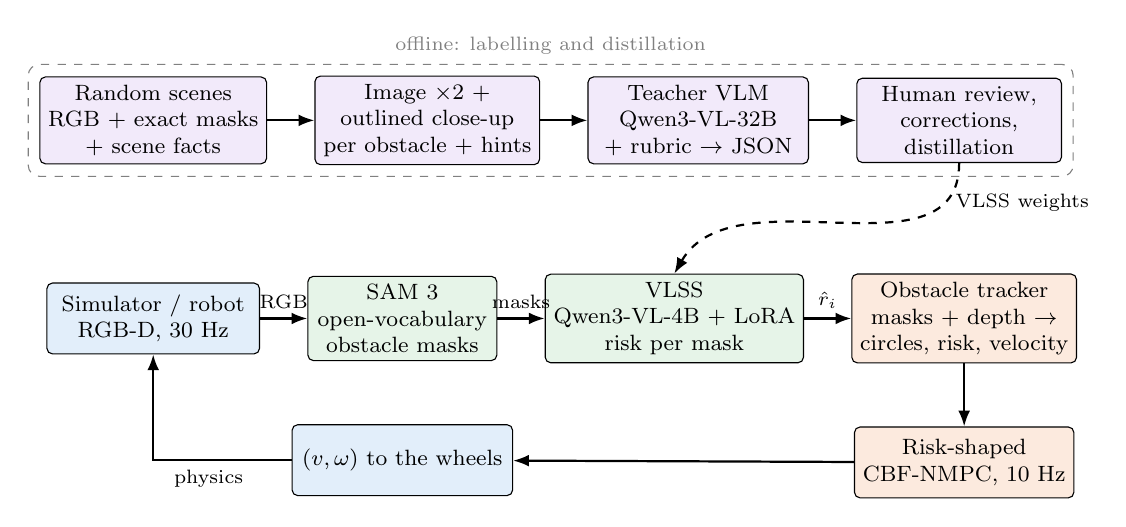
\begin{tikzpicture}[node distance=5mm and 6mm]
\node[box,fill=sim,minimum width=27mm] (sim) {Simulator / robot\\RGB-D, 30 Hz};
\node[box,fill=per,right=of sim,minimum width=24mm] (sam) {SAM 3\\open-vocabulary\\obstacle masks};
\node[box,fill=per,right=of sam,minimum width=28mm] (vls) {VLSS\\Qwen3-VL-4B + LoRA\\risk per mask};
\node[box,fill=ctl,right=of vls,minimum width=26mm] (trk) {Obstacle tracker\\masks + depth $\to$\\circles, risk, velocity};
\node[box,fill=ctl,below=8mm of trk,minimum width=26mm] (mpc) {Risk-shaped\\CBF-NMPC, 10 Hz};
\node[box,fill=sim,below=8mm of sam,minimum width=28mm] (cmd) {$(v,\omega)$ to the wheels};
\draw[arr] (sim) -- node[above,lab]{RGB} (sam);
\draw[arr] (sam) -- node[above,lab]{masks} (vls);
\draw[arr] (vls) -- node[above,lab]{$\hat r_i$} (trk);
\draw[arr] (trk) -- (mpc);
\draw[arr] (mpc) -- (cmd);
\draw[arr] (cmd.west) -| node[pos=0.3,below,lab]{physics} (sim.south);
\node[box,fill=off,above=15mm of sim,minimum width=27mm] (lay) {Random scenes\\RGB + exact masks\\+ scene facts};
\node[box,fill=off,right=of lay,minimum width=24mm] (cu) {Image $\times2$ +\\outlined close-up\\per obstacle + hints};
\node[box,fill=off,right=of cu,minimum width=28mm] (tea) {Teacher VLM\\Qwen3-VL-32B\\+ rubric $\to$ JSON};
\node[box,fill=off,right=of tea,minimum width=26mm] (rev) {Human review,\\corrections,\\distillation};
\draw[arr] (lay) -- (cu); \draw[arr] (cu) -- (tea); \draw[arr] (tea) -- (rev);
\draw[arr,dashed] (rev.south) to[out=-90,in=60] node[right,lab,pos=0.15]{VLSS weights} (vls.north);
\begin{scope}[on background layer]
\node[draw=gray,dashed,rounded corners,fit=(lay)(cu)(tea)(rev),inner sep=4pt,label={[font=\scriptsize,gray]above:offline: labelling and distillation}] {};
\end{scope}
\end{tikzpicture}}
\caption{Overview. Offline (top), the teacher sees the camera image and, per obstacle, a close-up with that obstacle outlined from
the simulator's exact mask, plus hints about what stands on it; its ratings are reviewed, corrected and distilled into VLSS.
At runtime (bottom), VLSS sees the camera image and SAM~3's masks.}
\label{fig:overview}
\end{figure}

\subsection{Why output a safety score and not safe actions}\label{sec:why}
An alternative is a VLA that maps images directly to safe actions, aligned with safety constraints during
training~\cite{zhang2025safevla}. We output a score per obstacle for six reasons.
\begin{enumerate}
\item \textbf{Guarantees stay with the controller.} The score enters a barrier function; the contact constraint is independent of it.
A wrong score makes the robot more or less cautious; it cannot command a collision (R1). A learned action policy offers no such
floor unless it is itself wrapped in a filter, which again needs to know what is risky.
\item \textbf{Failures are local and inspectable.} A wrong score belongs to one obstacle and can be seen, reviewed and corrected
(Section~\ref{sec:teacher}); an unsafe action is the product of the whole policy.
\item \textbf{Embodiment independence.} The same scores serve a differential-drive robot, a quadruped or a manipulator's motion
planner; only the controller changes. An action model must be retrained per embodiment.
\item \textbf{Data efficiency.} Labels are one number per object per image, produced automatically by a teacher; safe actions need
demonstrations or reinforcement learning with constraint costs per embodiment and environment.
\item \textbf{Rate decoupling.} Risk changes slowly; geometry changes fast. The scorer can run at a few hertz while the tracker
and controller run at control rate on depth; an action model must run at control rate.
\item \textbf{Composability.} Scores compose with any goal, planner or task, and with other safety layers (e.g.\ human-specified
constraints~\cite{feng2025words,santos2025updating}).
\end{enumerate}
The cost is a perception pipeline between the scorer and the controller (segmentation, depth, tracking), which can fail on its own
(Section~\ref{sec:closed}), and the loss of interaction semantics that only actions express (e.g.\ that a door may be pushed).

\subsection{Open-vocabulary obstacle segmentation with SAM~3}\label{sec:sam}
SAM~3~\cite{carion2026sam3} segments all instances of a concept named by a short text prompt. Its image detector
(Figure~\ref{fig:sam3}) is a DETR-style model~\cite{carion2020detr}: a 32-layer Perception Encoder ViT on a 1008$\times$1008 input
(patch 14, $72\times72$ tokens, windowed attention with global attention every 8 layers, 454~M parameters), a 24-layer text encoder
(354~M), a 6-layer encoder that fuses image and text features, and a 6-layer decoder with 200 object queries and a presence token.
For query $j$ and prompt $c$,
\begin{equation}
s_{j,c} = \sigma(\ell^{\text{presence}}_{c})\;\sigma(\ell^{\text{match}}_{j,c}),
\end{equation}
which separates whether the concept is in the image from where it is.

\begin{figure}[htbp]
\centering
\resizebox{\textwidth}{!}{%
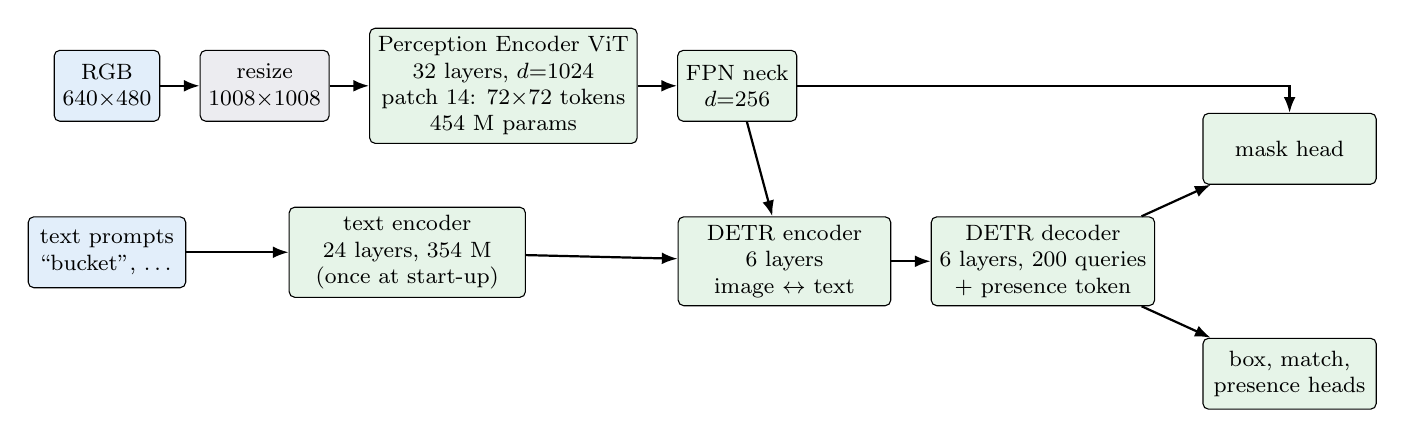
\begin{tikzpicture}[node distance=4mm and 5mm]
\node[box,fill=sim] (img) {RGB\\640$\times$480};
\node[box,fill=frz,right=of img] (rs) {resize\\1008$\times$1008};
\node[box,fill=per,right=of rs,minimum width=30mm] (vit) {Perception Encoder ViT\\32 layers, $d{=}1024$\\patch 14: $72{\times}72$ tokens\\454~M params};
\node[box,fill=per,right=of vit] (fpn) {FPN neck\\$d{=}256$};
\node[box,fill=sim,below=12mm of img,minimum width=20mm] (txt) {text prompts\\``bucket'', \dots};
\node[box,fill=per,right=of txt,minimum width=30mm,xshift=8mm] (te) {text encoder\\24 layers, 354~M\\(once at start-up)};
\node[box,fill=per,below=12mm of fpn,minimum width=27mm,xshift=6mm] (enc) {DETR encoder\\6 layers\\image $\leftrightarrow$ text};
\node[box,fill=per,right=of enc,minimum width=27mm] (dec) {DETR decoder\\6 layers, 200 queries\\+ presence token};
\node[box,fill=per,above right=4mm and 6mm of dec,minimum width=22mm] (mh) {mask head};
\node[box,fill=per,below right=4mm and 6mm of dec,minimum width=22mm] (bh) {box, match,\\presence heads};
\draw[arr] (img) -- (rs); \draw[arr] (rs) -- (vit); \draw[arr] (vit) -- (fpn); \draw[arr] (fpn) -- (enc);
\draw[arr] (txt) -- (te); \draw[arr] (te) -- (enc);
\draw[arr] (enc) -- (dec); \draw[arr] (dec) -- (bh); \draw[arr] (dec) -- (mh); \draw[arr] (fpn.east) -| (mh.north);
\end{tikzpicture}}
\caption{SAM~3 image detector. Image features are computed once per frame and shared by all prompts; text features once at start-up.}
\label{fig:sam3}
\end{figure}

\paragraph{Input resolution.} SAM~3's processor resizes every image to 1008$\times$1008, without keeping the aspect ratio. Our
simulated camera renders 640$\times$480, a choice made for rendering speed and for the scorer's token budget (300 image tokens),
so SAM~3 receives an upsampled image with no more detail than the original. A real OAK-D Pro colour sensor (12~MP, commonly
streamed at 1080p or 4K) can give SAM~3 a 1008-pixel input with real detail, which matters most for small objects such as a glass,
while VLSS keeps a 640$\times$480 copy.

\paragraph{Prompts and post-processing.} Nine prompts (\emph{bucket, drinking glass, glass vase, sofa, armchair, ottoman, bean bag,
person, robot}) run as one batch over shared image features; detections with $s\geq0.40$ are kept, mask probabilities are
thresholded at 0.5, masks of different prompts with IoU $\geq0.6$ are merged, and at most 40 are kept. With
\code{torch.compile}: 49~ms per frame.

\paragraph{Obstacle test.} Each mask pixel $(u,v)$ with depth $z$ is back-projected with the intrinsics $K$ and the camera pose
$(R,t)$, $\bm p_w = R\,zK^{-1}[u,v,1]^\top + t$; a detection is an obstacle if the 2nd percentile of its points' heights is below the
robot's height (0.35~m). This removes the glass on a bucket or in a hand, and keeps a sofa when its legs are hidden.

\subsection{Teacher labels with privileged information}\label{sec:teacher}

\paragraph{Input.} The teacher, Qwen3-VL-32B~\cite{bai2025qwen3vl} (FP8, served with vLLM~\cite{kwon2023vllm}), receives per frame
(Figure~\ref{fig:teacher}): the rubric as system prompt (Appendix~\ref{app:rubric}); the camera image enlarged twice; one close-up per
obstacle, cut around it with one obstacle height of margin above, enlarged to about 512~px, \emph{with that obstacle outlined} from
the simulator's exact mask; scene hints (``obstacle 2 has a drinking glass standing on it''); and a JSON schema. It does not receive
a masked-out image: risk depends on context (what stands on the obstacle, who stands in front of it), which masking would remove;
the outline marks which object is meant while keeping the context. Exact masks rather than SAM~3's keep segmentation errors out of
the labels.

\paragraph{Output.} JSON per obstacle: a name, what it carries, four booleans (soft, fragile, carries fragile, living), a reason and
the risk, in that order, so that the reason is written before the number~\cite{wang2024cot}. Decoding is greedy.

\begin{figure}[htbp]
\centering
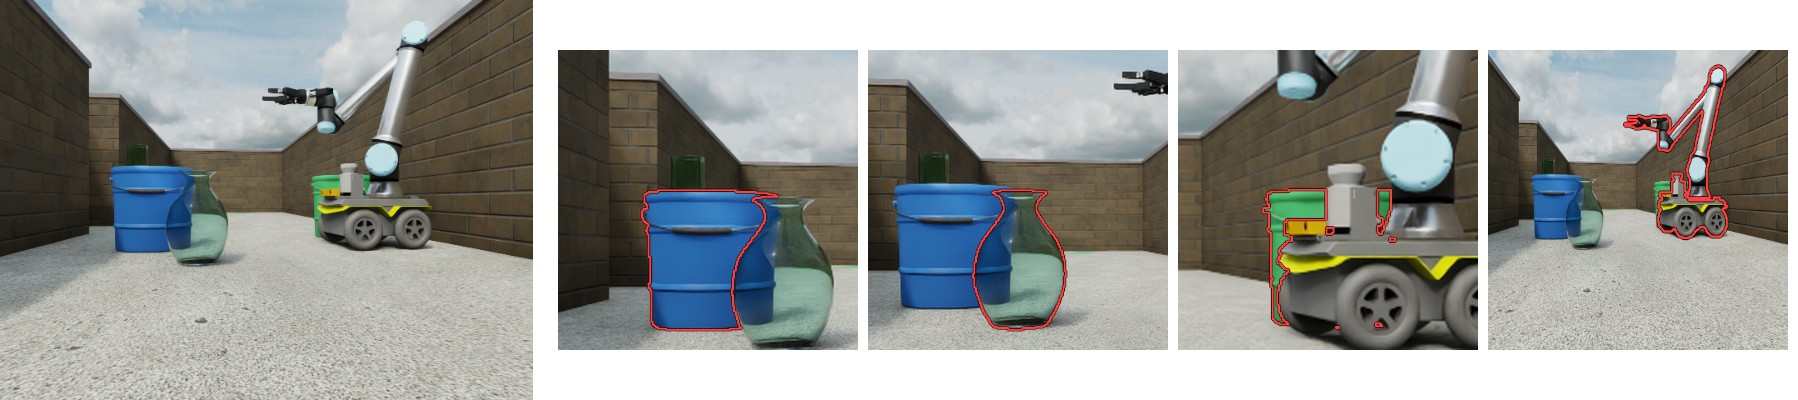
\includegraphics[width=\textwidth]{figures/teacher_input.jpg}
\caption{What the teacher sees for one frame: the camera image (left) and one close-up per obstacle with that obstacle outlined.
Teacher ratings for this frame, from left to right: bucket with a drinking glass on it 0.65 (``a bump could knock over the glass''),
glass vase on the floor 0.85, bucket 0.20, gripper robot 0.40 (corrected to 0.65 by the review).}
\label{fig:teacher}
\end{figure}

\paragraph{Privileged hints.} In a 64-frame pilot the teacher noticed the glass on a bucket lid in 27\,\% of frames with the image and
close-ups alone and in 55\,\% with 1920$\times$1440 renders; with hints from the simulator, in 100\,\%, with every such bucket
rated inside its range. The hints name things and never risks; VLSS never sees them.

\paragraph{Which obstacles are rated.} Objects with at least 300 visible pixels whose base is below 0.35~m and of which at least 25\,\%
is visible (pixel count over the silhouette area expected at that distance, $\approx f^2A/d^2$), unless they cover 4{,}000 pixels.

\paragraph{Review and correction.} A reviewer inspected 64 frames chosen to cover every semantic state and raised the policy for the
gripper robot and for glass on the floor. The corrected label follows from the teacher's $r$, the range of the obstacle's state and
whether the teacher's description names the object:
\begin{equation}
\tilde r = \begin{cases}
r_{\text{reviewer}} & \text{if the reviewer set it,}\\
r & \text{if } r\in[l_s,h_s],\\
\min(\max(r,l_s),h_s) & \text{if the teacher recognised the object,}\\
\operatorname{median}\{r' : \text{in-range ratings of state } s\} & \text{otherwise (it described a neighbour).}
\end{cases}
\end{equation}
Of 12{,}235 ratings, 9{,}943 were kept, 2{,}023 clipped, 258 replaced and 11 set by the reviewer. Within a range, the value remains the
teacher's.

\subsection{VLSS: the student scorer}\label{sec:student}

VLSS (Figure~\ref{fig:student}) is Qwen3-VL-4B-Instruct~\cite{bai2025qwen3vl} with a frozen vision encoder, LoRA~\cite{hu2022lora}
adapters on the language model, query tokens and a regression head. Its input is the RGB image, a fixed instruction and up to
$K=8$ obstacle masks; its output, per mask, is a risk $\hat r_k\in[0,1]$ and four attribute probabilities.

\begin{figure}[htbp]
\centering
\resizebox{\textwidth}{!}{%
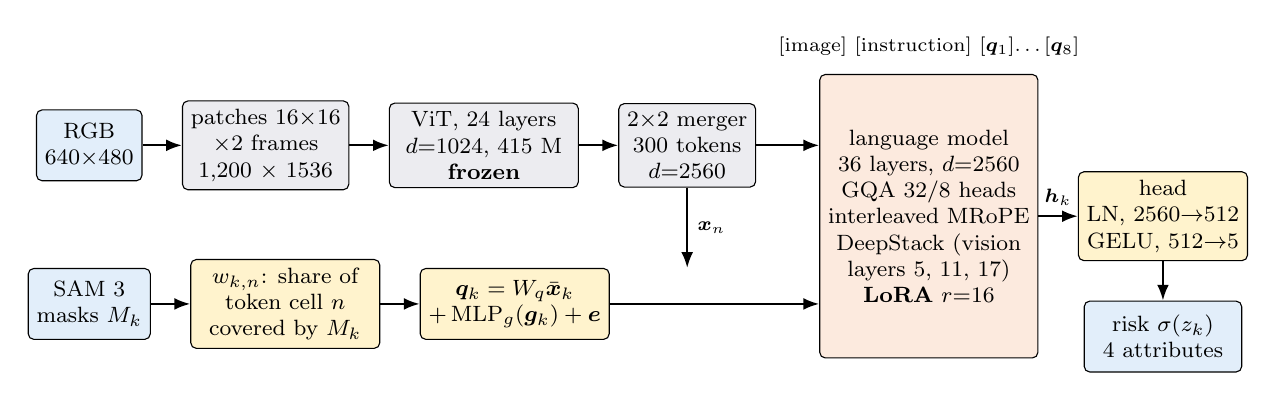
\begin{tikzpicture}[node distance=4mm and 5mm]
\node[box,fill=sim] (img) {RGB\\640$\times$480};
\node[box,fill=frz,right=of img] (pe) {patches $16{\times}16$\\$\times$2 frames\\1{,}200 $\times$ 1536};
\node[box,fill=frz,right=of pe,minimum width=24mm] (vit) {ViT, 24 layers\\$d{=}1024$, 415~M\\\textbf{frozen}};
\node[box,fill=frz,right=of vit] (mg) {$2{\times}2$ merger\\300 tokens\\$d{=}2560$};
\node[box,fill=sim,below=11mm of img] (msk) {SAM 3\\masks $M_k$};
\node[box,fill=trn,right=of msk,minimum width=24mm] (pool) {$w_{k,n}$: share of\\token cell $n$\\covered by $M_k$};
\node[box,fill=trn,right=of pool,minimum width=24mm] (q) {$\bm q_k = W_q\bar{\bm x}_k$\\$+\,\mathrm{MLP}_g(\bm g_k) + \bm e$};
\node[box,fill=ctl,right=8mm of mg,minimum height=36mm,minimum width=27mm,yshift=-9mm] (lm) {language model\\36 layers, $d{=}2560$\\GQA 32/8 heads\\interleaved MRoPE\\DeepStack (vision\\layers 5, 11, 17)\\\textbf{LoRA} $r{=}16$};
\node[box,fill=trn,right=of lm,minimum width=20mm] (hd) {head\\LN, 2560$\to$512\\GELU, 512$\to$5};
\node[box,fill=sim,below=5mm of hd,minimum width=20mm] (o) {risk $\sigma(z_k)$\\4 attributes};
\draw[arr] (img) -- (pe); \draw[arr] (pe) -- (vit); \draw[arr] (vit) -- (mg);
\draw[arr] (msk) -- (pool); \draw[arr] (pool) -- (q); \draw[arr] (mg.south) -- node[right,lab]{$\bm x_n$} (q.north -| mg.south);
\draw[arr] (mg.east) -- (lm.west |- mg.east); \draw[arr] (q.east) -- (lm.west |- q.east);
\draw[arr] (lm) -- node[above,lab]{$\bm h_k$} (hd); \draw[arr] (hd) -- (o);
\node[lab,above=1mm of lm] {[image] [instruction] [$\bm q_1$]\dots[$\bm q_8$]};
\end{tikzpicture}}
\caption{VLSS. Grey: frozen; yellow: trained from scratch; orange: frozen weights with trained LoRA adapters. One forward pass, no
text generation.}
\label{fig:student}
\end{figure}

\paragraph{Image tokens.} The image is cut into $16\times16$ patches, duplicated in time (Qwen3-VL treats an image as a two-frame
video): 1{,}200 vectors of 1536 values, encoded by 24 transformer layers and merged in $2\times2$ groups into $N=300$ tokens
$\bm x_n\in\R^{2560}$, each covering a $32\times32$-pixel cell $C_n$.

\paragraph{Query tokens.} For mask $M_k$:
\begin{equation}
w_{k,n} = \frac{|M_k\cap C_n|}{|C_n|},\qquad
\bar{\bm x}_k = \frac{\sum_n w_{k,n}\,\bm x_n}{\sum_n w_{k,n}},\qquad
\bm q_k = W_q\,\bar{\bm x}_k + \mathrm{MLP}_g(\bm g_k) + \bm e,
\end{equation}
with geometry $\bm g_k=(u_0,v_0,u_1,v_1,\sqrt a,\bar u,\bar v,v_{98})\in[0,1]^8$ (box, square root of the area fraction, centroid,
98th-percentile row, normalised by the image size). $W_q$ starts as the identity, the last layer of $\mathrm{MLP}_g$ as zero and $\bm e$
as the embedding of an unused token, so each query starts as its object's mean feature.

\paragraph{Attention.} The language model reads the sequence (image tokens, instruction, $\bm q_1,\dots,\bm q_8$) with causal
attention,
\begin{equation}
\mathrm{Attn}(Q,K,V)=\mathrm{softmax}\Big(\frac{QK^\top}{\sqrt{d_h}}+C\Big)V,\qquad C_{ij}=\begin{cases}0 & j\leq i\\ -\infty & j>i.\end{cases}
\end{equation}
Each query attends to the whole
image and the instruction, so a bucket's score can use the pixels of the glass on it, outside the bucket's mask. Unused query slots
come last and cannot affect used ones. DeepStack~\cite{meng2024deepstack} adds features of vision layers 5, 11 and 17 to the
first three language layers.

\paragraph{Head and adapters.} $[z_k,\bm a_k]=W_2\,\mathrm{GELU}(W_1\,\mathrm{LN}(\bm h_k))$, $\hat r_k=\sigma(z_k)$,
$\hat{\bm\alpha}_k=\sigma(\bm a_k)$ for \emph{soft, fragile, carries fragile, living}. Every attention and MLP projection of the
language model gets $W'=W+\frac{\alpha}{r}BA$ with $r=16$, $\alpha=32$. Trainable: 41.6~M of 4.48~B parameters. For inference the
adapters are merged. Qwen3-VL's patch embedding, a \code{Conv3d} whose kernel equals its stride, took 5~s per image in bfloat16 on
our GPU; it is replaced by the identical matrix product (difference $3\cdot10^{-6}$).

\subsection{Training objective}\label{sec:training}
A sample is a frame with up to 8 rated obstacles. Each obstacle's mask is SAM~3's own (precomputed, matched at IoU $\geq0.5$) with
probability 0.8 when SAM~3 found it, otherwise the exact mask, so VLSS learns on the masks it gets at runtime. Augmentation:
horizontal flip ($p=0.5$) and per-channel gain and offset ($\pm15\,\%$). With targets $\tilde r_k$, teacher attributes
$\bm\alpha_k$ and valid queries $\mathcal V$:
\begin{align}
\mathcal L_{\text{risk}} &= \frac{1}{|\mathcal V|}\sum_{k\in\mathcal V}\frac{1}{\delta}\,\mathrm{Huber}_\delta(\hat r_k-\tilde r_k),\qquad \delta=0.1,\\
\mathcal L_{\text{rank}} &= \frac{1}{|\mathcal P|}\sum_{(i,j)\in\mathcal P}\log\big(1+e^{-(z_i-z_j)}\big),\qquad
\mathcal P=\{(i,j)\text{ in one frame}: \tilde r_i-\tilde r_j\geq0.10\},\\
\mathcal L_{\text{attr}} &= \frac{1}{4|\mathcal V|}\sum_{k\in\mathcal V}\sum_{m=1}^{4}\mathrm{BCE}(\hat\alpha_{k,m},\alpha_{k,m}),\qquad
\mathcal L = \mathcal L_{\text{risk}} + 0.5\,\mathcal L_{\text{rank}} + 0.2\,\mathcal L_{\text{attr}}.
\end{align}
The Huber term fits values, the ranking term the order within a frame (what the controller acts on), and the attribute term gives
the representation reasons. AdamW, $\eta(s)=\eta_0\min(1,\frac{s+1}{100})\frac12(1+\cos\frac{\pi s}{S})$ with $\eta_0=2\cdot10^{-4}$,
weight decay 0.01, batch 8, 4 epochs, bfloat16; the checkpoint with the lowest validation MAE is kept.

\subsection{Risk-shaped CBF-NMPC}\label{sec:nmpc}

\paragraph{Model and cost.} State $\bm x=[p_x,p_y,\theta,v,\omega]^\top$, input $\bm u=[a,\alpha]^\top$,
$\dot{\bm x}=[v\cos\theta,v\sin\theta,\omega,a,\alpha]^\top$, discretised with RK4, $\Delta t=0.12$~s, $N=25$; solved with
IPOPT~\cite{waechter2006ipopt} through CasADi~\cite{andersson2019casadi} at 10~Hz, warm-started. With goal $\bm g$ and slacks
$s_{i,k}\geq0$:
\begin{equation}
J=\sum_{k=0}^{N-1}\Big(\|\bm p_{k+1}-\bm g\|^2 + 0.3\,p_{y,k+1}^2 + 0.5\,a_k^2 + 0.05\,\alpha_k^2 + 0.2\,\omega_{k+1}^2\Big)
+ 20\,\|\bm p_N-\bm g\|^2 + \sum_{i,k}\big(200\,s_{i,k}^2 + 20\,s_{i,k}\big),
\end{equation}
with velocity, acceleration and wall bounds on $k\geq1$ (bounding the measured initial state made 40\,\% of problems infeasible).

\paragraph{Barriers.} For obstacle circle $i$ predicted at constant velocity,
$d_{i,k}=\|\bm p_k-(\bm c_i+k\Delta t\,\bm v_i)\|$ and $h_{i,k}=d_{i,k}-(\rho+R_i+m(r_i))$:
\begin{align}
&d_{i,k+1}\geq\rho+R_i+m_0 &&\text{(contact, hard, independent of the risk; } m_0=0.01\text{ m)}\\
&h_{i,k+1}\geq(1-\gamma(r_i))\,h_{i,k}-s_{i,k} &&\text{(discrete-time CBF~\cite{zeng2021dcbf}, soft)}\\
&m(r)=0.03+0.32\,r\text{ m},\quad \gamma(r)=0.70-0.55\,r. &&
\end{align}
Without slack, $h_{i,k}\geq(1-\gamma)^k h_{i,0}$: a robot outside the risk margin stays outside (forward invariance), and one inside
can approach only geometrically slowly. A sofa ($r\approx0.07$) may be passed 5~cm away and approached quickly ($\gamma=0.66$); a
person ($r\approx0.95$) is kept 33~cm away and approached slowly ($\gamma=0.18$). The slack lets the risk margin give way where space
is short, in proportion to its penalty, never the contact constraint (R1, R2). $h$ is in metres: with squared distances a large
obstacle dominated a small one of higher risk. Figure~\ref{fig:constraints} illustrates the two constraints.

\begin{figure}[htbp]
\centering
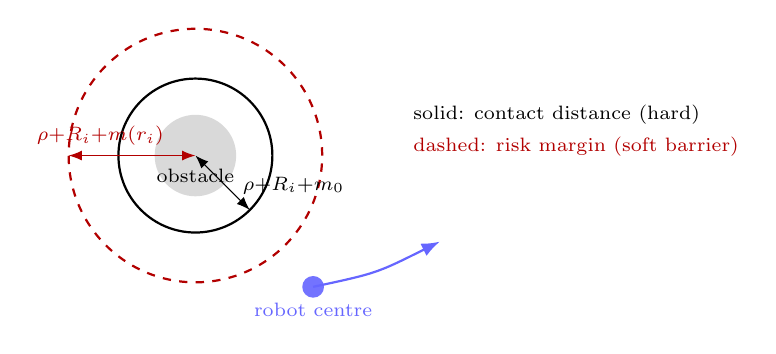
\begin{tikzpicture}[scale=1.15]
\fill[gray!30] (0,0) circle (0.45); \node[font=\scriptsize] at (0,-0.22) {obstacle};
\draw[thick] (0,0) circle (0.85);
\draw[dashed,thick,red!70!black] (0,0) circle (1.4);
\draw[{Latex}-{Latex}] (0,0) -- (0.6,-0.6) node[pos=0.55,right,font=\scriptsize,xshift=1mm]{$\rho{+}R_i{+}m_0$};
\draw[{Latex}-{Latex},red!70!black] (0,0) -- (-1.4,0) node[pos=0.75,above,font=\scriptsize]{$\rho{+}R_i{+}m(r_i)$};
\node[font=\scriptsize,anchor=west] at (2.3,0.45) {solid: contact distance (hard)};
\node[font=\scriptsize,anchor=west,red!70!black] at (2.3,0.1) {dashed: risk margin (soft barrier)};
\fill[blue!55] (1.3,-1.45) circle (0.12);
\draw[-{Latex},blue!60,thick] (1.3,-1.45) .. controls (2.0,-1.3) .. (2.7,-0.95);
\node[font=\scriptsize,blue!60] at (1.3,-1.7) {robot centre};
\end{tikzpicture}
\caption{The two constraints around one obstacle; the robot's radius $\rho$ is added to the obstacle's.}
\label{fig:constraints}
\end{figure}

\paragraph{Tracker.} Depth pixels of each obstacle mask between 2~cm and 0.35~m above the floor are projected to the floor and
down-sampled on a 4~cm grid. A detection joins the track with a floor point within 0.35~m; a still track accumulates points (it stays
known outside the field of view), a moving one keeps only the latest; velocity and risk are exponential averages (factor 0.3).
Each track's points are split along their main axis into pieces of at most 0.3~m, each covered by a circle plus 5~cm. Low points no
mask covers become unknown obstacles with risk 0.7.

%======================================================================================================================
\section{Experimental setup}\label{sec:setup}

\subsection{Simulator, robot and scenarios}
Isaac Sim 5.1 and Isaac Lab~\cite{mittal2023orbit}; PhysX at 120~Hz, sensors and control at 30~Hz. The test environment is an
8~m$\times$2.2~m walled alley (Figure~\ref{fig:scene}a) chosen to force gaps between obstacles of very different risk: two buckets,
a drinking glass, a glass vase, a sofa, an armchair, an ottoman and a bean bag, all dynamic rigid bodies. The robot is a TurtleBot~4
driven through its wheel joints (Create~3 limits: 0.46~m/s, 1.9~rad/s, 0.9~m/s$^2$, 4~rad/s$^2$; $\rho=0.172$~m) with an OAK-D Pro
camera model (640$\times$480, 69$^\circ$, 24~cm above the floor). In the \emph{person} scenario an animated person carries the glass
from one bucket to the other while the robot drives past; in the \emph{gripper robot} scenario a Jackal with a UR10e arm and a
Robotiq 2F-140 gripper does the same (Figure~\ref{fig:scene}b).

\begin{figure}[htbp]
\centering
\begin{subfigure}[t]{0.32\textwidth}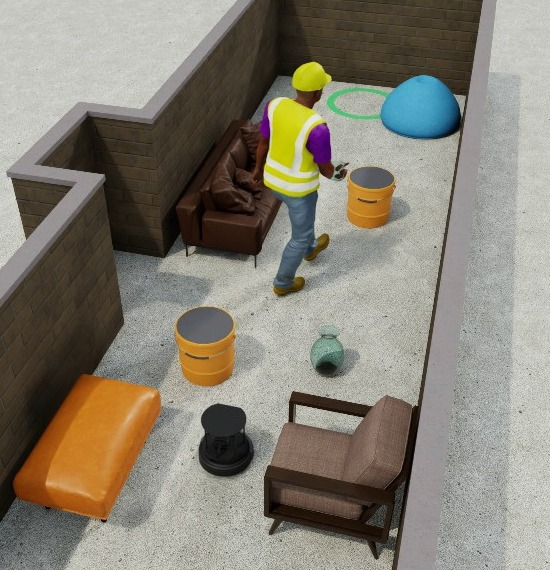
\includegraphics[width=\linewidth]{figures/person_t09_overview_crop.jpg}\caption{Person scenario.}\end{subfigure}\hfill
\begin{subfigure}[t]{0.32\textwidth}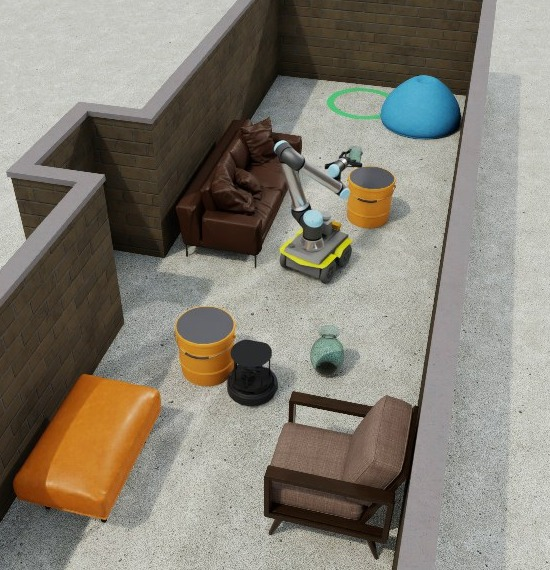
\includegraphics[width=\linewidth]{figures/gripper_t12_overview_crop.jpg}\caption{Gripper-robot scenario.}\end{subfigure}\hfill
\begin{subfigure}[t]{0.32\textwidth}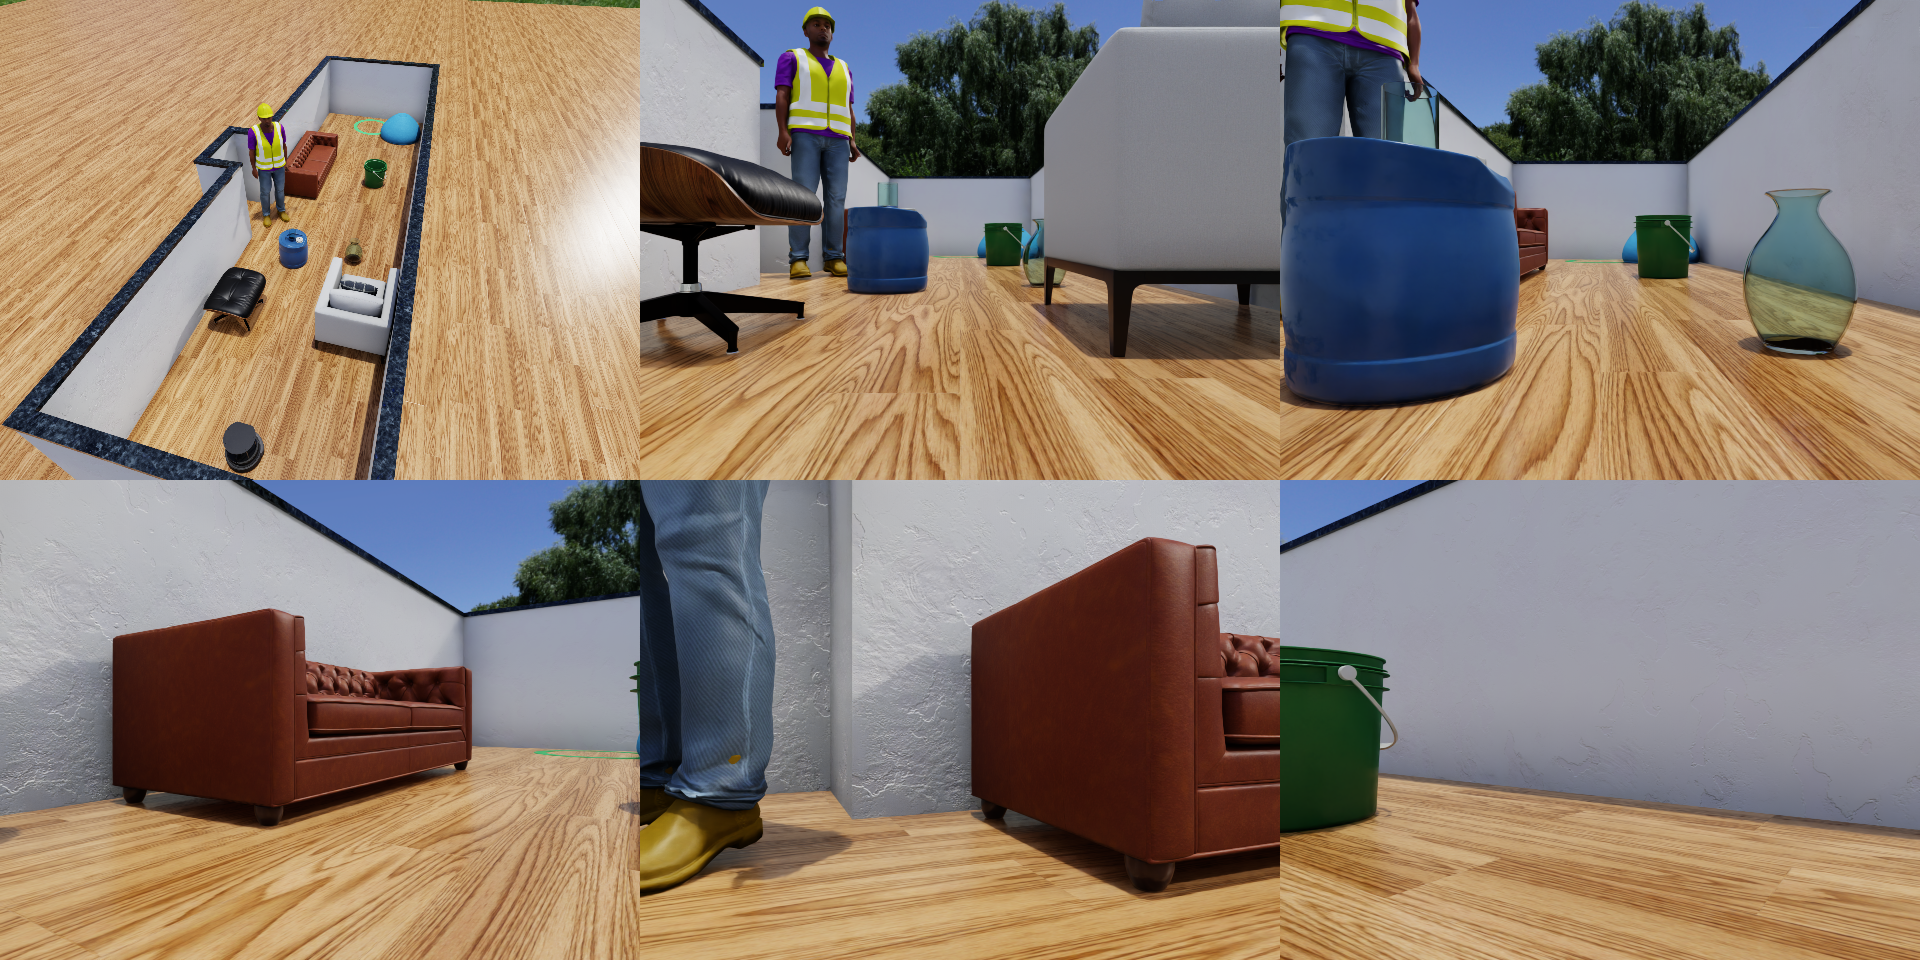
\includegraphics[width=\linewidth]{figures/ood_scene.png}\caption{Unseen scene.}\end{subfigure}
\caption{Simulation environments. (a, b) The test alley with the two actors that move the glass. (c) The unseen scene: other
containers, sofa, armchair, ottoman, floor, walls and sky (top left: overview; others: robot camera).}
\label{fig:scene}
\end{figure}

\subsection{Scene generation and its validity}\label{sec:layouts}
Random scenes are produced by a layout sampler (\code{envs/layout.py}) and applied by the simulator. The sampler places objects in
two roles. \emph{Floor objects} (furniture, containers, the bean bag, and the glass or vase when on the floor) are placed one by one,
largest first, at random poses (furniture mostly against a wall), and a pose is accepted only if the object's footprint polygon lies
inside the alley and keeps at least 0.10~m from every footprint already placed (separating-axis test). \emph{Carried objects} (only
the glass and the vase) are placed on a support chosen from a whitelist: a bucket lid, a seat, or the actor's hand. Supports offer
measured surfaces: a lid's radius, and for seats the flat spots of the cushion found from the furniture model's mesh (the 30th
percentile of surface height over the seat area; spots within 2.5~cm of it, so never on a throw pillow or an armrest). Large objects
are never carried, so physically meaningless arrangements such as a table on a vase cannot be generated. After placement the physics
runs for 0.5~s, and the support relations written to the dataset are recomputed from the settled poses, not taken from the plan; in
a check of the extra layouts, no glass or vase ended neither on its support nor on the floor. Robot viewpoints are sampled 0.55--3.8~m
from an object with at least 0.06~m clearance. Figure~\ref{fig:layouts} shows examples. The sampler does not judge plausibility
beyond these rules; for new object categories a scene grammar and a physics acceptance test (reject a layout if anything moves or
tips while settling) would be needed.

\begin{figure}[htbp]
\centering
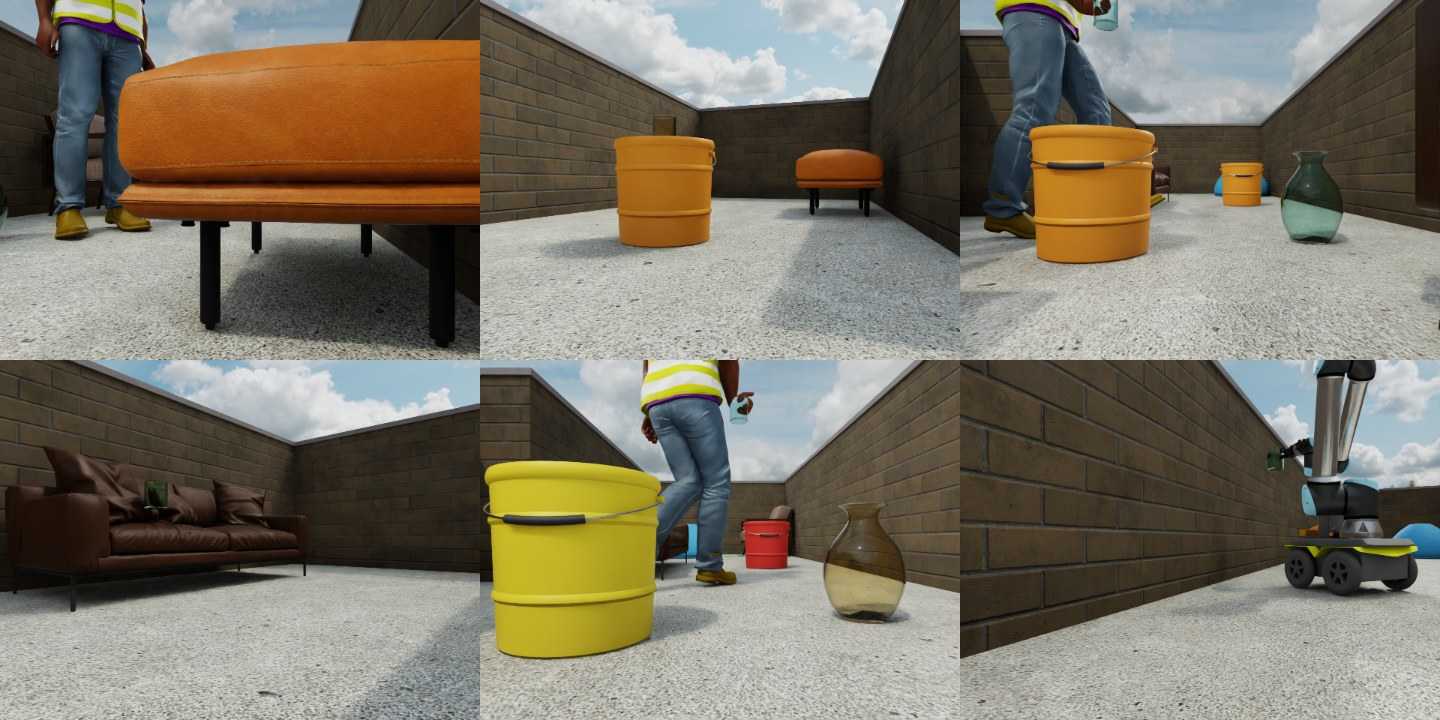
\includegraphics[width=\textwidth]{figures/layouts.jpg}
\caption{Robot-camera frames from random scenes: ottoman; glass on a bucket; person holding the glass; glass on the sofa seat;
vase on the floor; gripper robot holding the glass.}
\label{fig:layouts}
\end{figure}

\subsection{Datasets}
Per scenario: 130 random static scenes seen from 12 viewpoints, 48 extra scenes with the glass or vase on the sofa or armchair seat
(added for VLSS v2), and 6 driving episodes of the scripted transfer (a frame every 0.5~s). Splits are assigned per scene
(Table~\ref{tab:splits}); \code{test\_heldout} contains an arrangement no other split has: the glass or vase on the ottoman. The
\emph{unseen scene} (Figure~\ref{fig:scene}c, 1{,}152 frames from 96 random layouts) replaces the containers by two warehouse pails,
the furniture by a Chesterfield sofa, a white upholstered armchair and a leather swivel ottoman, and the floor, walls and sky.

\begin{table}[htbp]
\centering\small
\caption{Frames per split (12{,}235 rated obstacles in total).}
\label{tab:splits}
\begin{tabular}{lrrrrr}
\toprule
 & train & val & test & test\_heldout & total \\
\midrule
frames & 4{,}031 & 336 & 452 & 240 & 5{,}059 \\
\bottomrule
\end{tabular}
\end{table}

\subsection{Metrics and protocols}
Against labels: mean absolute error (MAE), the share within 0.10, and pair accuracy, the share of pairs in $\mathcal P$ ranked the right
way. Against the policy (no labels needed): a score is \emph{inside} when $\hat r\in[l_s-0.05,h_s+0.05]$. Every test runs with SAM~3's
masks (what the robot sees) and with exact masks. Closed loop: minimum gap between the robot's disc and each footprint, contacts,
where the glass ends, time to the goal, solver statistics; with simulator obstacles under policy risks (midpoint of each range) and
under one uniform risk of 0.5, and with the full pipeline. Gate for deployment: test MAE $\leq0.08$, pair accuracy $\geq90\,\%$,
latency $\leq50$~ms. Hardware: one NVIDIA RTX PRO 6000 Blackwell (96~GB), AMD Threadripper PRO 9975WX.

\begin{table}[htbp]
\centering\small
\caption{Models: size, input and output.}
\label{tab:models}
\begin{tabularx}{\textwidth}{>{\raggedright}p{2.6cm}>{\raggedright}p{2.3cm}>{\raggedright}X>{\raggedright\arraybackslash}p{4.2cm}}
\toprule
Model & Size & Input & Output \\
\midrule
SAM~3 & 0.86~B, 1.7~GB & RGB (resized to 1008$\times$1008), 9 text prompts & mask, box and score per instance \\
Teacher: Qwen3-VL-32B (FP8) & 33~B, 36~GB & rubric, image $\times$2, close-up per obstacle, hints, JSON schema & JSON per obstacle: name, carries, 4 booleans, reason, risk \\
VLSS: Qwen3-VL-4B + LoRA + head & 4.48~B (42~M trained), 9~GB & RGB 640$\times$480, instruction, $\leq8$ masks & risk and 4 attribute probabilities per mask \\
CBF-NMPC & $N=25$, $\leq16$ circles & state, goal, scored circles & $(v,\omega)$ \\
\bottomrule
\end{tabularx}
\end{table}

%======================================================================================================================
\section{Results}\label{sec:results}

\subsection{Accuracy against the reviewed labels}
Table~\ref{tab:labels} compares VLSS v1, trained when only buckets ever carried anything, with v2, trained with the extra scenes. v2
passes the gate on unseen layouts (MAE 0.052, pair accuracy 99.6\,\%) and the MAE part on the held-out arrangement (0.077; pair
accuracy 89.3\,\%). With exact masks the numbers change by at most 0.001: SAM~3's masks cost VLSS almost nothing.

\begin{table}[htbp]
\centering\small
\caption{VLSS against the corrected labels, with SAM~3's masks.}
\label{tab:labels}
\begin{tabular}{lrcccccc}
\toprule
 & & \multicolumn{3}{c}{v1} & \multicolumn{3}{c}{v2} \\
\cmidrule(lr){3-5}\cmidrule(lr){6-8}
Split & obstacles & MAE & within 0.10 & pairs & MAE & within 0.10 & pairs \\
\midrule
val & 744 & 0.070 & 84.5\,\% & 96.1\,\% & 0.057 & 86.0\,\% & 98.4\,\% \\
test & 1{,}051 & 0.066 & 83.2\,\% & 97.1\,\% & \textbf{0.052} & 85.3\,\% & \textbf{99.6\,\%} \\
test\_heldout & 480 & 0.137 & 79.2\,\% & 80.6\,\% & \textbf{0.077} & 85.0\,\% & \textbf{89.3\,\%} \\
\bottomrule
\end{tabular}
\end{table}

\subsection{Generalisation to held-out arrangements and an unseen scene}
Table~\ref{tab:policyeval} reports mean scores per semantic state against the policy. In the unseen scene both models keep their
behaviour on new containers, furniture and materials (92--94\,\% of scores inside the ranges, against 89--92\,\% on the normal test
frames); v2 rates the new white armchair 0.19, slightly above its range. Something fragile on a support never seen carrying anything,
the ottoman, is recognised only by v2, and only partly: 0.51 on \code{test\_heldout} (v1 0.08, range 0.60--0.85) and 0.76 in the
unseen scene (v1 0.22, 7 cases). Figure~\ref{fig:qual} shows the difference in the driving video.

\begin{table}[htbp]
\centering\small
\caption{Mean scores per semantic state, normal test frames and the unseen scene.}
\label{tab:policyeval}
\begin{tabular}{lcrccrcc}
\toprule
 & & \multicolumn{3}{c}{test + test\_heldout} & \multicolumn{3}{c}{unseen scene} \\
\cmidrule(lr){3-5}\cmidrule(lr){6-8}
Semantic state & range & $n$ & v1 & v2 & $n$ & v1 & v2 \\
\midrule
armchair & 0.00--0.15 & 143 & 0.12 & 0.15 & 302 & 0.15 & 0.19 \\
couch & 0.00--0.15 & 195 & 0.10 & 0.12 & 313 & 0.12 & 0.14 \\
ottoman & 0.00--0.15 & 79 & 0.06 & 0.06 & 62 & 0.21 & 0.18 \\
bean bag & 0.00--0.15 & 142 & 0.05 & 0.05 & 193 & 0.04 & 0.05 \\
bucket & 0.15--0.35 & 374 & 0.24 & 0.23 & 483 & 0.23 & 0.22 \\
gripper robot & 0.65--0.75 & 102 & 0.67 & 0.67 & 167 & 0.68 & 0.68 \\
bucket + drinking glass & 0.60--0.85 & 93 & 0.80 & 0.80 & 197 & 0.70 & 0.69 \\
bucket + glass vase & 0.60--0.85 & 16 & 0.70 & 0.78 & 83 & 0.76 & 0.73 \\
armchair or couch + glass or vase & 0.60--0.85 & 32 & 0.12 & 0.70 & -- & -- & -- \\
ottoman + glass or vase (held out) & 0.60--0.85 & 71 & 0.08 & 0.51 & 7 & 0.22 & 0.76 \\
glass vase on the floor & 0.80--0.90 & 84 & 0.88 & 0.87 & 192 & 0.89 & 0.88 \\
drinking glass on the floor & 0.80--0.90 & 13 & 0.85 & 0.86 & 40 & 0.87 & 0.87 \\
gripper robot + glass & 0.80--0.90 & 28 & 0.79 & 0.80 & 27 & 0.79 & 0.80 \\
person (with or without the glass) & 0.90--1.00 & 159 & 1.00 & 1.00 & 207 & 1.00 & 1.00 \\
\midrule
\multicolumn{2}{l}{share inside the range} & 1{,}531 & 89.2\,\% & \textbf{92.4\,\%} & 2{,}273 & 93.7\,\% & \textbf{91.9\,\%} \\
\bottomrule
\end{tabular}
\end{table}

\begin{figure}[htbp]
\centering
\begin{subfigure}[t]{0.32\textwidth}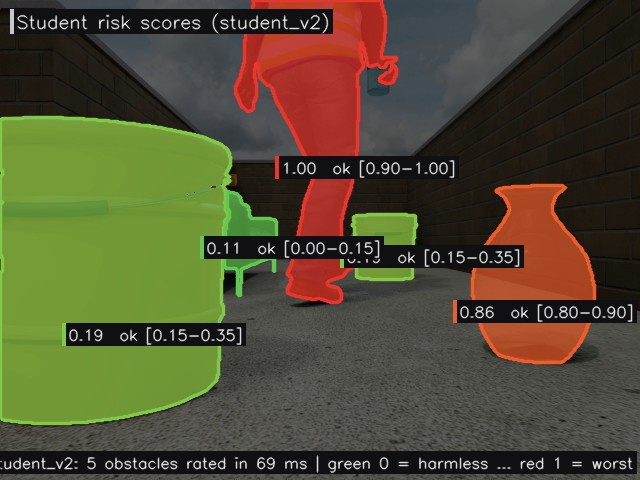
\includegraphics[width=\linewidth]{figures/person_t09_risk.jpg}\caption{Person scenario, v2.}\end{subfigure}\hfill
\begin{subfigure}[t]{0.32\textwidth}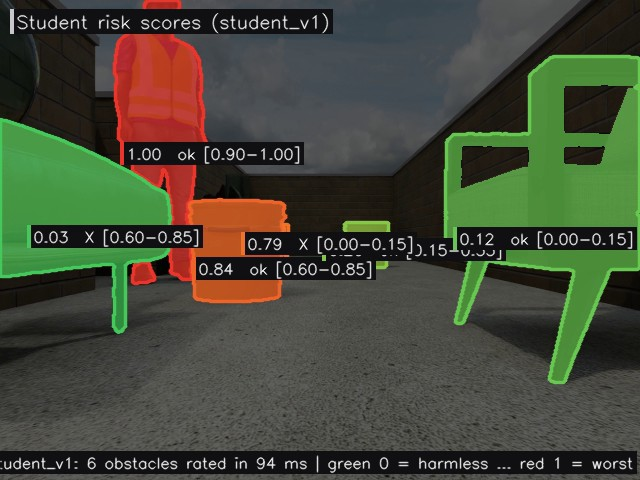
\includegraphics[width=\linewidth]{figures/ottoman_v1_t03_risk.jpg}\caption{Vase on the ottoman, v1.}\end{subfigure}\hfill
\begin{subfigure}[t]{0.32\textwidth}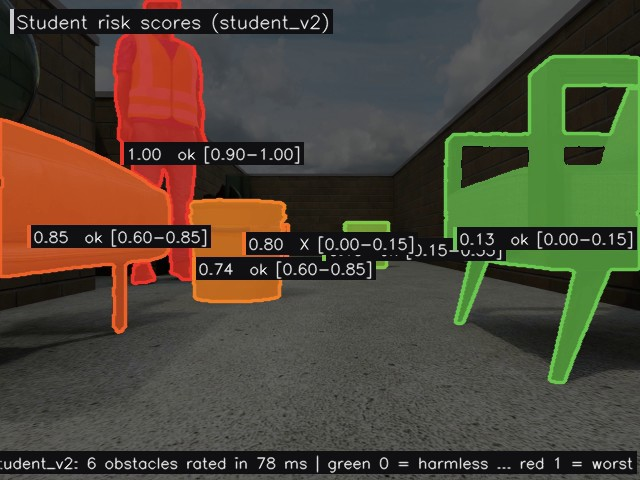
\includegraphics[width=\linewidth]{figures/ottoman_v2_t03_risk.jpg}\caption{Vase on the ottoman, v2.}\end{subfigure}
\caption{VLSS scores on SAM~3 masks in driving videos (green 0, red 1), with the policy range and whether the score is inside it.
(a) The person 1.00, the vase on the floor 0.86, buckets 0.19 and the armchair 0.11. (b, c) The ottoman with the vase (left edge),
an arrangement held out of training: v1 rates it as a plain ottoman, v2 at 0.85.}
\label{fig:qual}
\end{figure}

\subsection{Closed-loop navigation}\label{sec:closed}
Table~\ref{tab:closed} and Figure~\ref{fig:topview} compare semantic and uniform risk with simulator obstacles. In a kinematic test
(ideal unicycle, same layout), semantic risk passes the sofa at $p_y=+0.06$ with 0.16~m to the bucket carrying the glass, uniform risk
passes in the middle with 0.01~m. In Isaac Sim, in the person scenario, semantic risk gives the bucket with the glass ten times the
gap, the person more room, and uses the sofa as the side to hug, with the same time to the goal and no contact. In the gripper
scenario both runs touched the vase (1.7~cm overlap at $t=9.6$~s): the Jackal crossed in front of the robot, its constant-velocity
prediction left no feasible plan (20 solves not converged), and the controller executed the last unconverged iterate instead of braking.
With the full pipeline, the robot stopped 0.7~m after the start, between the ottoman and the armchair, without contact; the tracker's
circles, fitted to the visible fronts of the furniture with 5~cm padding, most likely closed the 0.7~m-wide passage.

\begin{table}[htbp]
\centering\small
\caption{Closed-loop results in Isaac Sim: minimum gaps (m) between the robot's disc and each footprint.}
\label{tab:closed}
\begin{tabular}{llcccccc}
\toprule
Scenario & risk & goal & bucket + glass & sofa & person / robot & vase & converged \\
\midrule
person & uniform 0.5 & 23.6~s & 0.01 & 0.17 & 0.33 & 0.11 & 100\,\% \\
person & \textbf{semantic} & 23.3~s & \textbf{0.11} & \textbf{0.07} & \textbf{0.40} & 0.11 & 100\,\% \\
gripper robot & uniform 0.5 & 27.4~s & 0.11 & 0.62 & 0.12 & $-0.02$ & 93\,\% \\
gripper robot & semantic & 27.7~s & 0.11 & 0.05 & 0.25 & $-0.02$ & 93\,\% \\
person & full pipeline & not reached & -- & -- & 1.74 & -- & 96\,\% \\
gripper robot & full pipeline & not reached & -- & -- & 1.96 & -- & 88\,\% \\
\bottomrule
\end{tabular}
\end{table}

\begin{figure}[htbp]
\centering
\begin{subfigure}[t]{0.49\textwidth}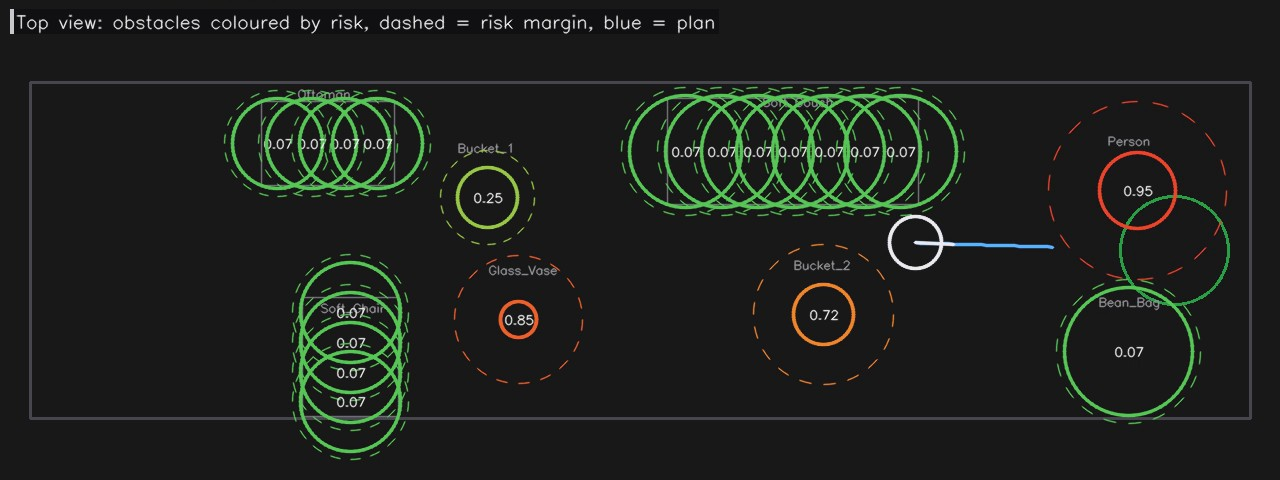
\includegraphics[width=\linewidth]{figures/nmpc_policy_person_default_t18_top.jpg}\caption{Semantic risk.}\end{subfigure}\hfill
\begin{subfigure}[t]{0.49\textwidth}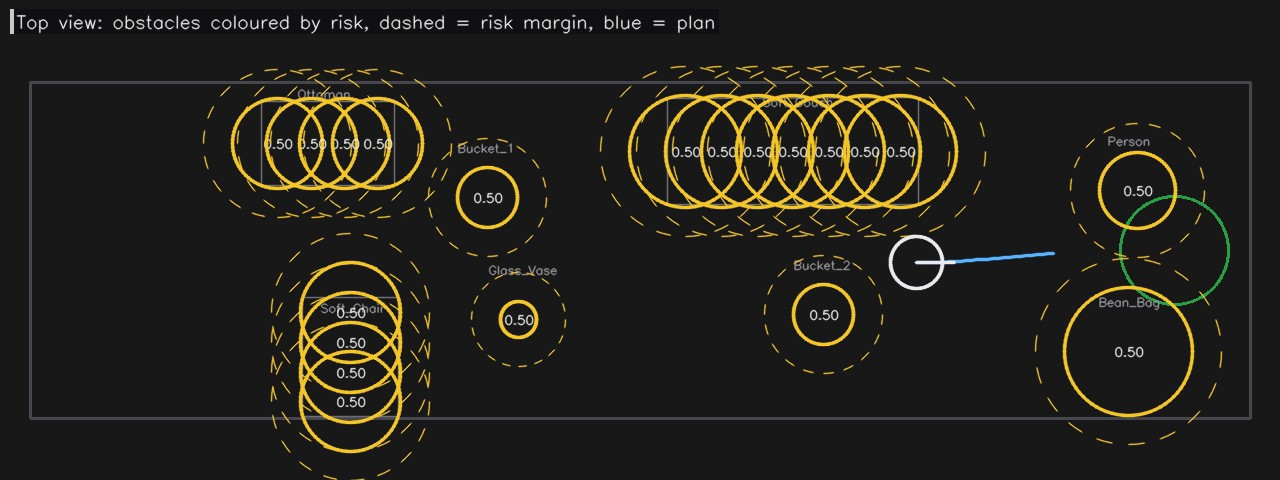
\includegraphics[width=\linewidth]{figures/nmpc_uniform_person_default_t18_top.jpg}\caption{Uniform risk 0.5.}\end{subfigure}
\caption{Top view at $t=18$~s in the person scenario. Circles: obstacles as the controller sees them, coloured by risk; dashed: risk
margin; white: robot; blue: plan. With semantic risk the margins of the sofa are thin and those of Bucket~2 (glass, 0.72), the vase
and the person wide.}
\label{fig:topview}
\end{figure}

\subsection{Runtime and embedded deployment}\label{sec:runtime}
Table~\ref{tab:runtime} lists measured times; Table~\ref{tab:jetson} estimates embedded rates from the compute per frame (VLSS: about
1.0~TFLOP in the vision encoder and 2.5~TFLOP in the language model; SAM~3: about 4.7~TFLOP), assuming 40\,\% of the dense FP16 tensor
throughput. These are estimates, not measurements. The present VLSS with SAM~3 is real time on a Jetson AGX Thor class device; on an
AGX Orin it would run near 2~Hz, usable only if the tracker carries scores between updates. A 0.8B student, TensorRT with INT8/FP8
weights and a lighter or lower-rate segmenter would be needed for 10~Hz on Orin.

\begin{table}[htbp]
\centering\small
\caption{Measured runtime on the workstation (one process per stage).}
\label{tab:runtime}
\begin{tabular}{lrrl}
\toprule
Stage & median & rate & note \\
\midrule
SAM~3, 9 prompts, compiled & 49~ms & 20~Hz & 70--99~ms with 3 runs sharing the GPU \\
VLSS v2, 6 obstacles, with preprocessing & 29~ms & 34~Hz & p95 30~ms \\
perception total & 78~ms & 13~Hz & \\
CBF-NMPC solve (IPOPT) & 24--28~ms & 10~Hz used & p95 37~ms \\
teacher (offline) & 1.45~s & & 4 requests in parallel \\
\bottomrule
\end{tabular}
\end{table}

\begin{table}[htbp]
\centering\small
\caption{Estimated per-frame latency on embedded devices (not measured).}
\label{tab:jetson}
\begin{tabular}{lcccccc}
\toprule
Device & memory & dense FP16 & VLSS 4B & SAM~3 & both & 0.8B student \\
\midrule
RTX PRO 6000 (measured) & 96~GB & -- & 29~ms & 49~ms & 13~Hz & 22~ms \\
Jetson AGX Thor & 128~GB & $\sim$250 TFLOPS & $\sim$35~ms & $\sim$50~ms & $\sim$10~Hz & $\sim$10~ms \\
Jetson AGX Orin 64~GB & 64~GB & $\sim$40 TFLOPS & $\sim$200~ms & $\sim$300~ms & $\sim$2~Hz & $\sim$40~ms \\
Jetson Orin NX 16~GB & 16~GB & $\sim$15 TFLOPS & $\sim$0.6~s & $\sim$0.8~s & $<$1~Hz & $\sim$110~ms \\
Jetson Orin Nano 8~GB & 8~GB & $\sim$8 TFLOPS & no fit (bf16) & $\sim$1.5~s & -- & $\sim$0.2~s \\
\bottomrule
\end{tabular}
\end{table}

%======================================================================================================================
\section{Discussion and limitations}\label{sec:discussion}
\begin{itemize}
\item \textbf{One test environment.} Training data comes from one alley with two container models, one sofa, one armchair, one
ottoman, one glass and one vase. The unseen scene changes objects and materials but not the task's structure, and real images have
not been tested. Other domains (Table~\ref{tab:domains}) need their own prompts, rubric and object library.
\item \textbf{Privileged teacher.} Without hints the teacher missed most glasses on lids; labelling real images needs another source
of support relations (multi-view checks, human review).
\item \textbf{Labels are a policy.} The ranges encode one reviewer's judgement; VLSS reproduces the policy, not a measured outcome.
Breakage is not simulated.
\item \textbf{Partial relational generalisation.} v2 scores the held-out ottoman with a glass 0.51 (59\,\% inside): far better than v1,
not solved. Training covers three kinds of support.
\item \textbf{Closed set of prompts.} Anything SAM~3 is not prompted for becomes an unknown obstacle from depth with a fixed risk.
\item \textbf{Guarantees and the full loop.} The barrier guarantee needs a feasible problem and known obstacles; circles are fitted to
visible fronts and motion is extrapolated at constant velocity. The full pipeline does not yet reach the goal, and an infeasible
problem led to contact because the controller did not brake.
\item \textbf{Compute.} Real time only on workstation- or Thor-class hardware without further work.
\end{itemize}

%======================================================================================================================
\section{Conclusion and future work}
We distilled a 33B-parameter VLM's per-obstacle risk judgement, with privileged scene information and human review, into a 4B
vision-language safety scorer that rates every obstacle mask in one 29~ms pass, and used the scores to shape the margin and decay
rate of discrete-time barriers in NMPC while keeping a risk-independent contact constraint. The scorer is accurate on unseen layouts,
robust to new furniture, containers and materials, and partly generalises the relation ``fragile thing on top''; in closed loop with
simulator obstacles, semantic risk moves clearance from the sofa to the bucket that carries the glass at no cost in time.

Next steps: (1) fix the tracker so that the full loop reaches the goal, add a braking fallback and a contact-only emergency layer, and
evaluate over many random scenes; (2) draw every object category from a pool of models and hold out whole families, add more supports
and carried objects, and add other domains such as an industrial workplace; (3) open-vocabulary prompts with teacher ratings of
whatever is segmented; (4) real robot-height images with a real test set; (5) calibrate the policy with counterfactual bumps in
simulation, in the spirit of physics-informed world models~\cite{li2025pinwm}; (6) a 0.8B student and barriers on richer geometry
such as Gaussian splatting maps~\cite{chen2025safersplat,tscholl2025collisioncone}.

%======================================================================================================================
\begin{thebibliography}{99}\small

\bibitem{ames2019cbf} A.~D. Ames, S.~Coogan, M.~Egerstedt, G.~Notomista, K.~Sreenath, and P.~Tabuada, ``Control barrier functions: Theory and applications,'' in \emph{Proc. European Control Conference (ECC)}, 2019.
\bibitem{zeng2021dcbf} J.~Zeng, B.~Zhang, and K.~Sreenath, ``Safety-critical model predictive control with discrete-time control barrier function,'' in \emph{Proc. American Control Conference (ACC)}, 2021.
\bibitem{chen2025splatnav} T.~Chen, O.~Shorinwa, et al., ``Splat-Nav: Safe real-time robot navigation in Gaussian splatting maps,'' \emph{IEEE Transactions on Robotics}, vol.~41, pp.~2765--2784, 2025, arXiv:2403.02751.
\bibitem{chen2025safersplat} T.~Chen, A.~Swann, J.~Yu, O.~Shorinwa, R.~Murai, M.~Kennedy~III, and M.~Schwager, ``SAFER-Splat: A control barrier function for safe navigation with online Gaussian splatting maps,'' in \emph{Proc. IEEE ICRA}, 2025, arXiv:2409.09868.
\bibitem{hong2026polymerge} J.~Hong, C.-Y. Chiu, S.~Fridovich-Keil, and G.~Chou, ``PolyMerge: Compressing 3D Gaussian splats with polytope coverings for provably safe resource-constrained navigation,'' arXiv:2606.16232, 2026.
\bibitem{tscholl2025collisioncone} D.~Tscholl, Y.~Nakka, and B.~Gunter, ``Perception-integrated safety critical control via analytic collision cone barrier functions on 3D Gaussian splatting,'' arXiv:2509.14421, 2025.
\bibitem{brunke2025semantic} L.~Brunke, Y.~Zhang, R.~R\"omer, J.~Naimer, N.~Staykov, S.~Zhou, and A.~P. Schoellig, ``Semantically safe robot manipulation: From semantic scene understanding to motion safeguards,'' \emph{IEEE Robotics and Automation Letters}, vol.~10, no.~5, pp.~4810--4817, 2025.
\bibitem{ravichandran2026core} Z.~Ravichandran, D.~Snyder, A.~Robey, H.~Hassani, V.~Kumar, and G.~J. Pappas, ``Contextual safety reasoning and grounding for open-world robots,'' arXiv:2602.19983, 2026.
\bibitem{feng2025words} Z.~Feng, H.~Zhang, and S.~Bansal, ``From words to safety: Language-conditioned safety filtering for robot navigation,'' arXiv:2511.05889, 2025.
\bibitem{santos2025updating} L.~Santos, Z.~Li, L.~Peters, S.~Bansal, and A.~Bajcsy, ``Updating robot safety representations online from natural language feedback,'' in \emph{Proc. IEEE ICRA}, 2025, arXiv:2409.14580.
\bibitem{chen2026alphaadj} J.~Chen and R.~Chandra, ``Dynamic control barrier function regulation with vision-language models for safe, adaptive, and realtime visual navigation,'' arXiv:2603.21142, 2026.
\bibitem{chen2026semanticcbf} J.~Chen and R.~Chandra, ``Semantically adaptive control barrier functions with vision-language models for real-time robot navigation,'' preprint (bibliographic details to be completed from the reference library).
\bibitem{kim2026predictive} T.~Kim, S.~Fradi, Y.~Dai, M.~Ostaszewski, and J.~Schmidhuber, ``Predictive semantic safety: From visual physical reasoning to safety-critical control,'' arXiv:2609.34356, 2026.
\bibitem{palanivelan_aerial} Palanivelan et al., ``VLM-guided semantic safety for onboard aerial autonomy,'' preprint (bibliographic details to be completed).
\bibitem{chen2025riskfields} T.~Chen, M.~Dominguez-Kuhne, A.~Swann, X.~Liu, and M.~Schwager, ``Semantic-metric Bayesian risk fields: Learning robot safety from human videos with a VLM prior,'' arXiv:2512.08233, 2025.
\bibitem{zhang2026semanticdf} D.~Zhang, N.~Chen, S.~Liu, R.~Tron, and Z.~Fan, ``Embedding semantic risk into distance fields and CBFs for online monocular safe control,'' arXiv:2606.01605, 2026.
\bibitem{khass2026semsafe} A.~M. Khass et al., ``SemSafe-3DGS: Semantic risk-aware active navigation in uncertain 3D Gaussian splatting maps,'' arXiv:2609.19330, 2026.
\bibitem{yang2026safesage} L.~Yang, R.~Bena, A.~D. Ames, et al., ``Safe-SAGE: Social-semantic adaptive guidance for safe engagement through Laplace-modulated Poisson safety functions,'' arXiv:2603.05497, 2026.
\bibitem{qian2024closing} J.~Qian, S.~Zhou, N.~J. Ren, V.~Chatrath, and A.~P. Schoellig, ``Closing the perception-action loop for semantically safe navigation in semi-static environments,'' in \emph{Proc. IEEE ICRA}, pp.~11641--11648, 2024.
\bibitem{lilja2026scenelm} A.~Lilja, F.~H\"ubel, S.~He, J.~Fu, C.~Tomlin, L.~Hammarstrand, J.~Malik, J.~Frey, and M.~Pavone, ``A scene language model for open-vocabulary scene mapping,'' arXiv:2609.21400, 2026.
\bibitem{pham2026semanticmapping} Pham et al., ``Efficient continuous semantic mapping based on spatio-temporal awareness,'' arXiv:2606.22672, 2026.
\bibitem{sinha2024aesop} R.~Sinha, A.~Elhafsi, C.~Agia, M.~Foutter, E.~Schmerling, and M.~Pavone, ``Real-time anomaly detection and reactive planning with large language models,'' in \emph{Proc. Robotics: Science and Systems (RSS)}, 2024.
\bibitem{potnis2026catnav} A.~Potnis, F.~Affonso, S.~Gummadi, N.~K. Uppalapati, and G.~Chowdhary, ``CATNAV: Cached vision-language traversability for efficient zero-shot robot navigation,'' arXiv:2603.22800, 2026.
\bibitem{baek_gating} Baek et al., ``Target-aware change detection for efficient VLM gating in mobile robots,'' preprint (bibliographic details to be completed).
\bibitem{wu_covnav} Wu et al., ``CovNav: Conformal prediction-guided adaptive inference for object goal navigation,'' preprint (bibliographic details to be completed).
\bibitem{wang2024cot} X.~Wang and D.~Zhou, ``Chain-of-thought reasoning without prompting,'' in \emph{Advances in Neural Information Processing Systems (NeurIPS)}, vol.~37, 2024.
\bibitem{zitkovich2023rt2} B.~Zitkovich et al., ``RT-2: Vision-language-action models transfer web knowledge to robotic control,'' in \emph{Proc. Conference on Robot Learning (CoRL)}, 2023.
\bibitem{kim2024openvla} M.~J. Kim et al., ``OpenVLA: An open-source vision-language-action model,'' in \emph{Proc. Conference on Robot Learning (CoRL)}, 2024.
\bibitem{zhang2025safevla} B.~Zhang, Y.~Zhang, J.~Ji, Y.~Lei, J.~Dai, Y.~Chen, and Y.~Yang, ``SafeVLA: Towards safety alignment of vision-language-action model via constrained learning,'' in \emph{Advances in Neural Information Processing Systems (NeurIPS)}, 2025, arXiv:2503.03480.
\bibitem{li2025pinwm} W.~Li, H.~Zhao, Z.~Yu, Y.~Du, Q.~Zou, R.~Hu, and K.~Xu, ``PIN-WM: Learning physics-informed world models for non-prehensile manipulation,'' in \emph{Proc. Robotics: Science and Systems (RSS)}, 2025.
\bibitem{carion2026sam3} N.~Carion et al., ``SAM 3: Segment anything with concepts,'' in \emph{Proc. International Conference on Learning Representations (ICLR)}, 2026, arXiv:2511.16719.
\bibitem{carion2020detr} N.~Carion, F.~Massa, G.~Synnaeve, N.~Usunier, A.~Kirillov, and S.~Zagoruyko, ``End-to-end object detection with transformers,'' in \emph{Proc. ECCV}, 2020.
\bibitem{bai2025qwen3vl} S.~Bai et al. (Qwen Team), ``Qwen3-VL technical report,'' arXiv:2511.21631, 2025.
\bibitem{meng2024deepstack} L.~Meng et al., ``DeepStack: Deeply stacking visual tokens is surprisingly simple and effective for LMMs,'' in \emph{Advances in Neural Information Processing Systems (NeurIPS)}, 2024.
\bibitem{hu2022lora} E.~J. Hu, Y.~Shen, P.~Wallis, Z.~Allen-Zhu, Y.~Li, S.~Wang, L.~Wang, and W.~Chen, ``LoRA: Low-rank adaptation of large language models,'' in \emph{Proc. ICLR}, 2022.
\bibitem{hinton2015distilling} G.~Hinton, O.~Vinyals, and J.~Dean, ``Distilling the knowledge in a neural network,'' arXiv:1503.02531, 2015.
\bibitem{kwon2023vllm} W.~Kwon et al., ``Efficient memory management for large language model serving with PagedAttention,'' in \emph{Proc. ACM SOSP}, 2023.
\bibitem{waechter2006ipopt} A.~W\"achter and L.~T. Biegler, ``On the implementation of an interior-point filter line-search algorithm for large-scale nonlinear programming,'' \emph{Mathematical Programming}, vol.~106, pp.~25--57, 2006.
\bibitem{andersson2019casadi} J.~A.~E. Andersson, J.~Gillis, G.~Horn, J.~B. Rawlings, and M.~Diehl, ``CasADi: A software framework for nonlinear optimization and optimal control,'' \emph{Mathematical Programming Computation}, vol.~11, pp.~1--36, 2019.
\bibitem{mittal2023orbit} M.~Mittal et al., ``Orbit: A unified simulation framework for interactive robot learning environments,'' \emph{IEEE Robotics and Automation Letters}, vol.~8, no.~6, pp.~3740--3747, 2023.
\end{thebibliography}

\appendix
\section{Rubric (version 2) given to the teacher}\label{app:rubric}
\begin{footnotesize}
You are the safety module of a TurtleBot 4, a small wheeled indoor robot: a disc 34 cm across and 34 cm tall that weighs about 4 kg and drives at up to 0.46 m/s (a third of walking pace). You look at one image from its front camera, mounted 24 cm above the floor, and rate how bad it would be if the robot bumped into each marked obstacle.

Risk is a number from 0.00 to 1.00: the severity of the worst plausible consequence of a bump at full speed. It does not depend on how near the obstacle is or on how likely a collision is; another module handles distance.

Consider, in this order:\\
1. People and animals. Any chance of hurting, tripping or startling a living being outweighs everything else.\\
2. What the obstacle carries. Look at what stands on it, lies in it, leans on it or is held by it. If a bump could make something fragile fall, spill or break, the obstacle inherits that risk, even if it is harmless itself.\\
3. The obstacle itself. Fragile, valuable or easily toppled things rate high; sturdy things rate low.\\
4. The robot. Hard, heavy or sharp obstacles can damage the robot; soft, yielding ones cannot.\\
5. Whether the damage can be undone. Broken glass is permanent; a pushed box is not.

Scale:\\
0.00-0.15 negligible. Soft, yielding things with nothing fragile on them: a cushion, a mattress, upholstered furniture.\\
0.15-0.35 minor. Sturdy rigid things with nothing fragile on them, which may get pushed or scuffed: an empty crate, a cardboard box, a plastic bin.\\
0.35-0.60 moderate. Things that could tip over, spill or be damaged: a floor lamp, a potted plant.\\
0.60-0.80 serious. Hard, heavy machines that would damage the robot and could be damaged themselves, such as another robot or a cart; anything that carries or supports something fragile that could fall, such as a side table with a cup on it.\\
0.80-0.90 very serious. Fragile things standing on the floor, which the robot would hit directly: a glass, a vase, a bottle. They will break or spill. A machine that is holding something fragile.\\
0.85-1.00 severe. People and animals, and anything whose failure could injure someone.

Judge only by what is visible in this image. If an obstacle seems to carry something but you cannot tell what, say so and rate it cautiously.

\textbf{Fields per obstacle, in this order:}
\begin{itemize}
\item \texttt{name}: what the obstacle is, 2 to 5 words
\item \texttt{carries}: what stands on it, lies in it or is held by it, as far as visible; ''nothing'' if nothing
\item \texttt{soft}: true if it yields when bumped (upholstery, fabric, foam)
\item \texttt{fragile}: true if the obstacle itself would probably break or be damaged
\item \texttt{carries\_fragile}: true if something fragile is on it, in it or held by it
\item \texttt{living}: true for people and animals
\item \texttt{reason}: the worst plausible consequence of a bump, at most 20 words
\item \texttt{risk}: 0.00 to 1.00, two decimals
\end{itemize}
\end{footnotesize}

\section{Main settings}\label{app:settings}
\begin{table}[H]
\centering\footnotesize
\caption{Settings used in all experiments.}
\label{tab:settings}
\begin{tabularx}{\textwidth}{l X}
\toprule
SAM~3 & score $\geq0.40$, mask 0.5, merge IoU 0.6, $\leq40$ detections, obstacle base $<0.35$~m, $\geq40$ depth points \\
Teacher & temperature 0, image $\times$2, close-ups 512~px, hints on, $\geq$300~px and $\geq$25\,\% visible \\
VLSS & $\leq$8 queries, LoRA $r=16$, $\alpha=32$, head 512, SAM~3 mask share 0.8, flip 0.5, colour jitter 0.15 \\
Training & AdamW $2\cdot10^{-4}$, weight decay 0.01, warm-up 100, cosine, batch 8, 4 epochs, loss weights 1 / 0.5 / 0.2, $\delta=0.1$ \\
NMPC & $N=25$, $\Delta t=0.12$~s, 10~Hz, $v\leq0.30$~m/s, $m\in[0.03,0.35]$~m, $\gamma\in[0.70,0.15]$, $m_0=0.01$~m, slack $200s^2+20s$ \\
Tracker & height 0.02--0.35~m, range 4~m, association 0.35~m, averaging 0.3, circles $\leq0.3$~m apart, pad 0.05~m, unknown risk 0.7 \\
\bottomrule
\end{tabularx}
\end{table}

\section{Code organisation}
\begin{table}[H]
\centering\footnotesize
\caption{Repository structure.}
\label{tab:repo}
\begin{tabularx}{\textwidth}{>{\ttfamily}l X}
\toprule
envs/ & simulator environment, scenarios, random layouts (\code{layout.py}), UR10e kinematics \\
perception/ & SAM~3 worker and client, obstacle test, VLSS worker and client, drawing \\
distillation/ & teacher requests, label corrections, VLSS model, data and metrics, progress files \\
control/ & CBF-NMPC (\code{cbf\_nmpc.py}) and the obstacle tracker (\code{obstacles.py}) \\
configs/ & environment (and the unseen scene), rubric and policy, VLSS, controller \\
scripts/ & dataset generation, labelling, training, evaluation, videos, tmux pipelines with progress bars \\
\bottomrule
\end{tabularx}
\end{table}

\end{document}
